\documentclass{article}\usepackage[]{graphicx}\usepackage[]{color}
%% maxwidth is the original width if it is less than linewidth
%% otherwise use linewidth (to make sure the graphics do not exceed the margin)
\makeatletter
\def\maxwidth{ %
  \ifdim\Gin@nat@width>\linewidth
    \linewidth
  \else
    \Gin@nat@width
  \fi
}
\makeatother

\definecolor{fgcolor}{rgb}{0.345, 0.345, 0.345}
\newcommand{\hlnum}[1]{\textcolor[rgb]{0.686,0.059,0.569}{#1}}%
\newcommand{\hlstr}[1]{\textcolor[rgb]{0.192,0.494,0.8}{#1}}%
\newcommand{\hlcom}[1]{\textcolor[rgb]{0.678,0.584,0.686}{\textit{#1}}}%
\newcommand{\hlopt}[1]{\textcolor[rgb]{0,0,0}{#1}}%
\newcommand{\hlstd}[1]{\textcolor[rgb]{0.345,0.345,0.345}{#1}}%
\newcommand{\hlkwa}[1]{\textcolor[rgb]{0.161,0.373,0.58}{\textbf{#1}}}%
\newcommand{\hlkwb}[1]{\textcolor[rgb]{0.69,0.353,0.396}{#1}}%
\newcommand{\hlkwc}[1]{\textcolor[rgb]{0.333,0.667,0.333}{#1}}%
\newcommand{\hlkwd}[1]{\textcolor[rgb]{0.737,0.353,0.396}{\textbf{#1}}}%
\let\hlipl\hlkwb

\usepackage{framed}
\makeatletter
\newenvironment{kframe}{%
 \def\at@end@of@kframe{}%
 \ifinner\ifhmode%
  \def\at@end@of@kframe{\end{minipage}}%
  \begin{minipage}{\columnwidth}%
 \fi\fi%
 \def\FrameCommand##1{\hskip\@totalleftmargin \hskip-\fboxsep
 \colorbox{shadecolor}{##1}\hskip-\fboxsep
     % There is no \\@totalrightmargin, so:
     \hskip-\linewidth \hskip-\@totalleftmargin \hskip\columnwidth}%
 \MakeFramed {\advance\hsize-\width
   \@totalleftmargin\z@ \linewidth\hsize
   \@setminipage}}%
 {\par\unskip\endMakeFramed%
 \at@end@of@kframe}
\makeatother

\definecolor{shadecolor}{rgb}{.97, .97, .97}
\definecolor{messagecolor}{rgb}{0, 0, 0}
\definecolor{warningcolor}{rgb}{1, 0, 1}
\definecolor{errorcolor}{rgb}{1, 0, 0}
\newenvironment{knitrout}{}{} % an empty environment to be redefined in TeX

\usepackage{alltt}
\usepackage[utf8]{inputenc}
\usepackage{hyperref}
\hypersetup{
  linktocpage,
  colorlinks=true, 
  linkcolor=blue,
  citecolor=blue,
  filecolor=blue,
  urlcolor=blue
}
\IfFileExists{upquote.sty}{\usepackage{upquote}}{}
\begin{document}

\title{Acetilation}
\author{Lucas Michel Todó}
\maketitle
\tableofcontents
\clearpage

\begin{knitrout}
\definecolor{shadecolor}{rgb}{0.969, 0.969, 0.969}\color{fgcolor}\begin{kframe}


{\ttfamily\noindent\itshape\color{messagecolor}{\#\# \\\#\# Attaching package: 'dplyr'}}

{\ttfamily\noindent\itshape\color{messagecolor}{\#\# The following objects are masked from 'package:stats':\\\#\# \\\#\#\ \ \ \  filter, lag}}

{\ttfamily\noindent\itshape\color{messagecolor}{\#\# The following objects are masked from 'package:base':\\\#\# \\\#\#\ \ \ \  intersect, setdiff, setequal, union}}\end{kframe}
\end{knitrout}


\section{Density Plots}
\subsection{log(Ac) All}
\begin{knitrout}
\definecolor{shadecolor}{rgb}{0.969, 0.969, 0.969}\color{fgcolor}
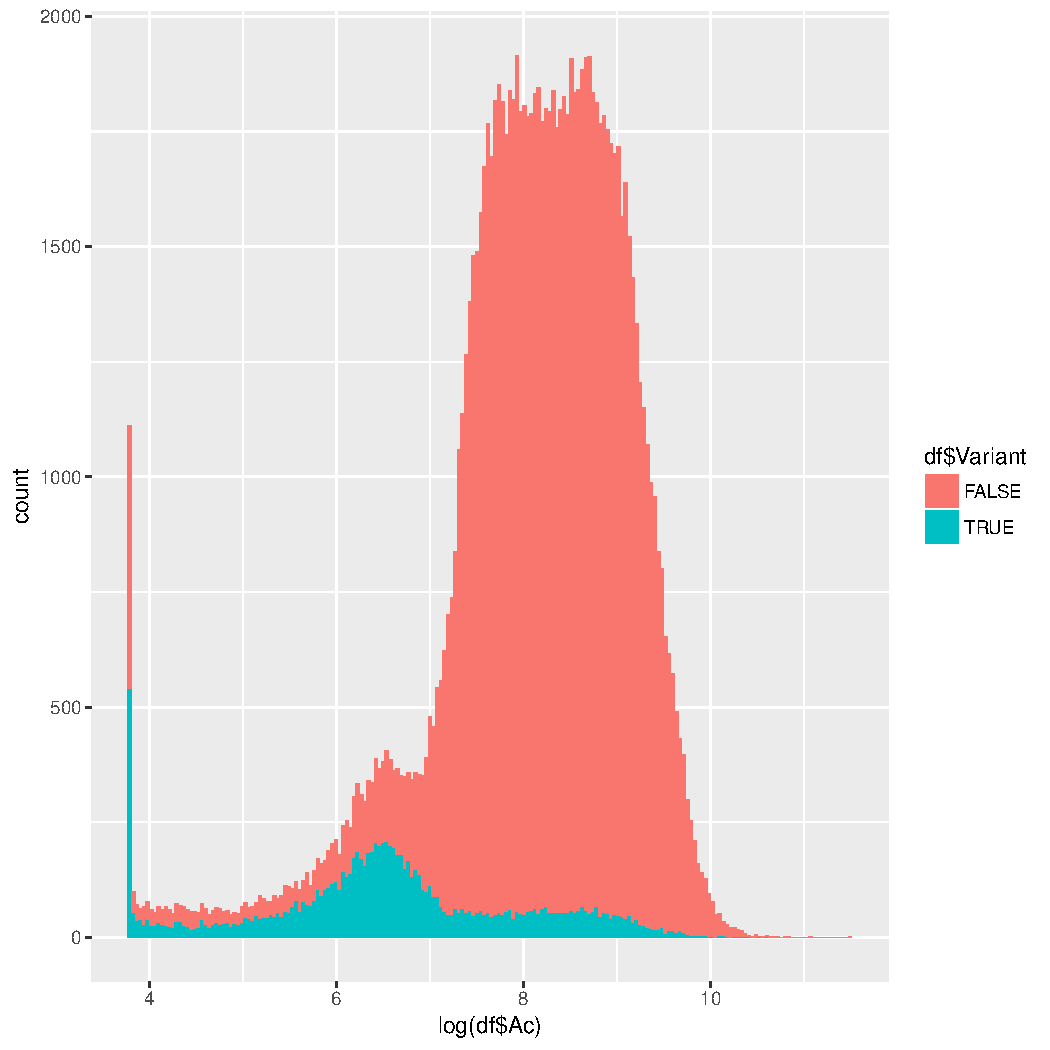
\includegraphics[width=1\linewidth]{figure/dens_all-1} 

\end{knitrout}
\clearpage
\subsection{log(Ac) 5'}
\begin{knitrout}
\definecolor{shadecolor}{rgb}{0.969, 0.969, 0.969}\color{fgcolor}
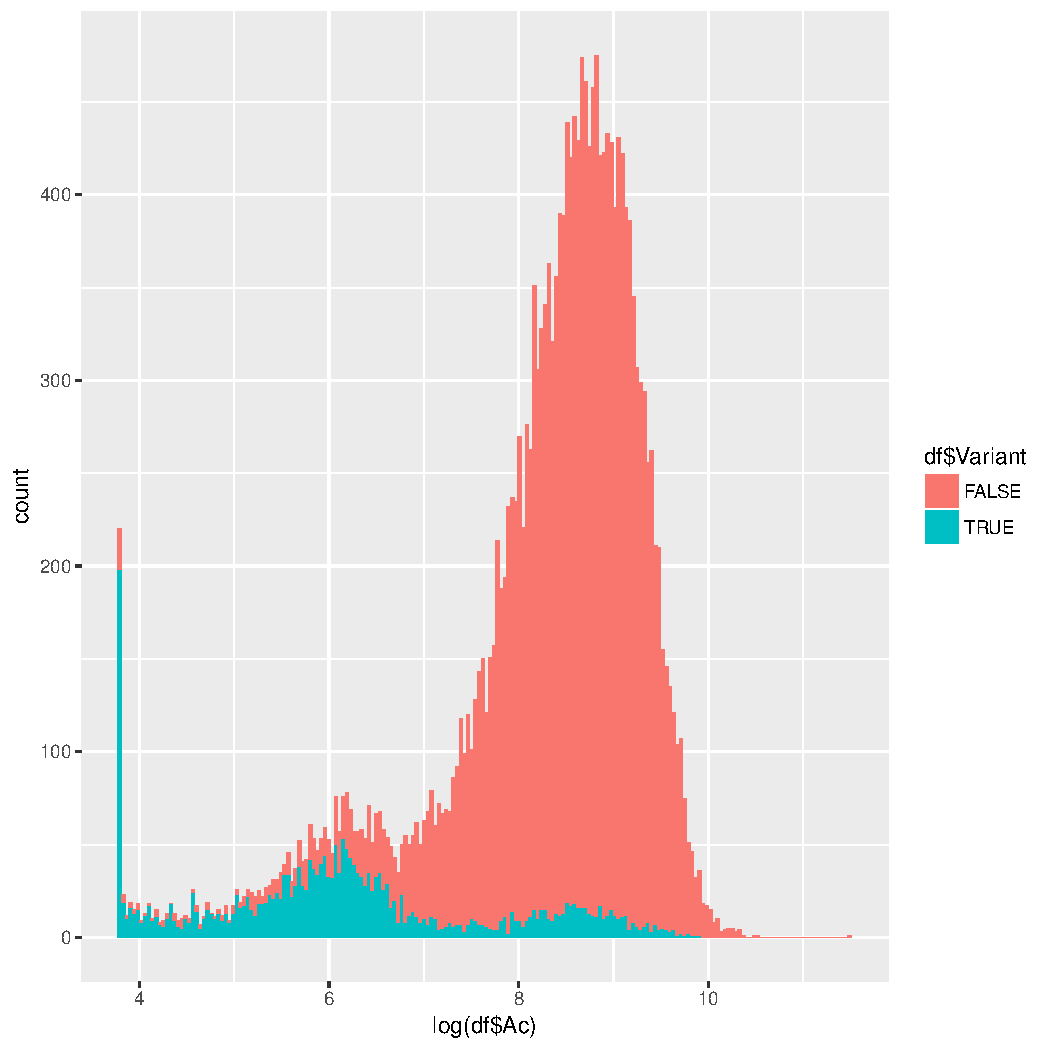
\includegraphics[width=1\linewidth]{figure/dens_5-1} 

\end{knitrout}
\clearpage
\subsection{log(Ac) ORF}
\begin{knitrout}
\definecolor{shadecolor}{rgb}{0.969, 0.969, 0.969}\color{fgcolor}
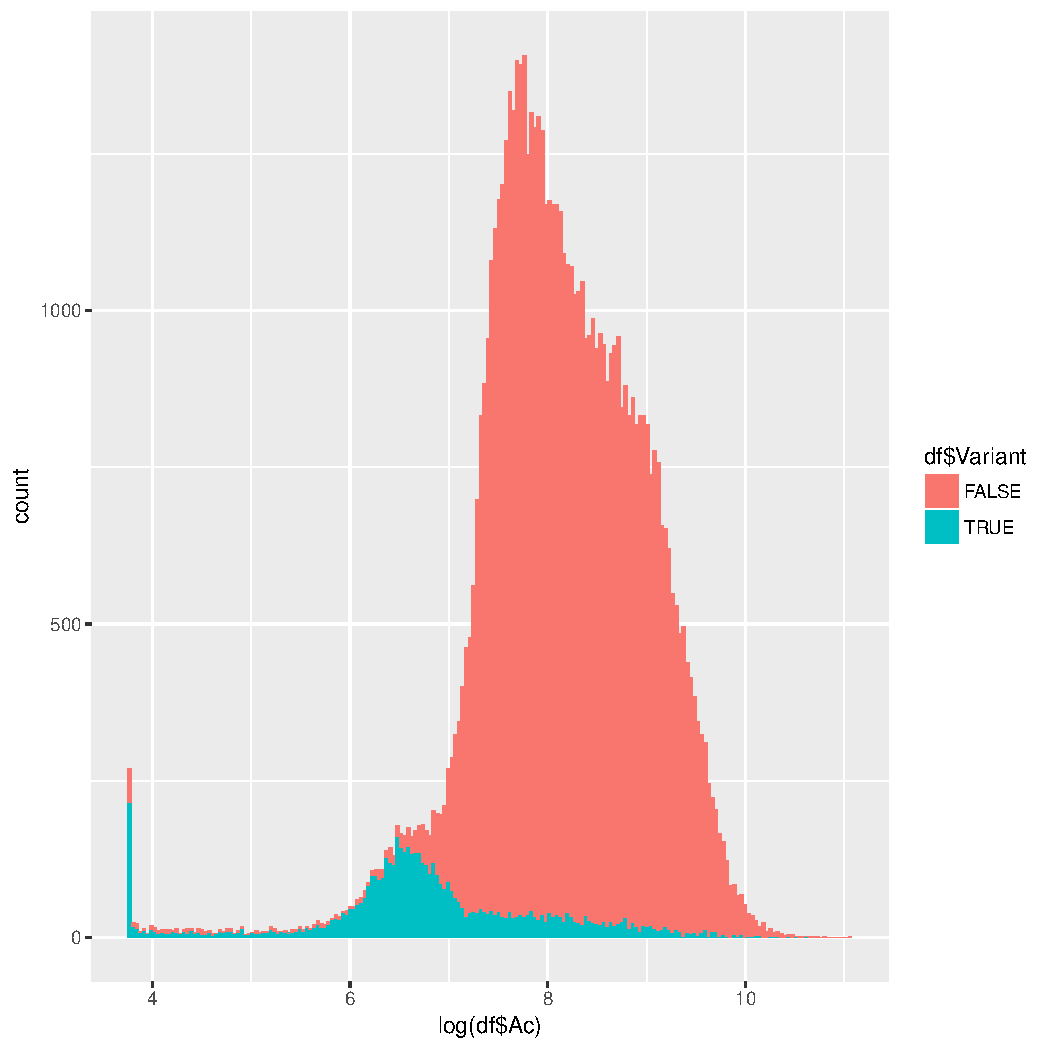
\includegraphics[width=1\linewidth]{figure/dens_ORF-1} 

\end{knitrout}
\clearpage
\subsection{log(Ac) 3'}
\begin{knitrout}
\definecolor{shadecolor}{rgb}{0.969, 0.969, 0.969}\color{fgcolor}
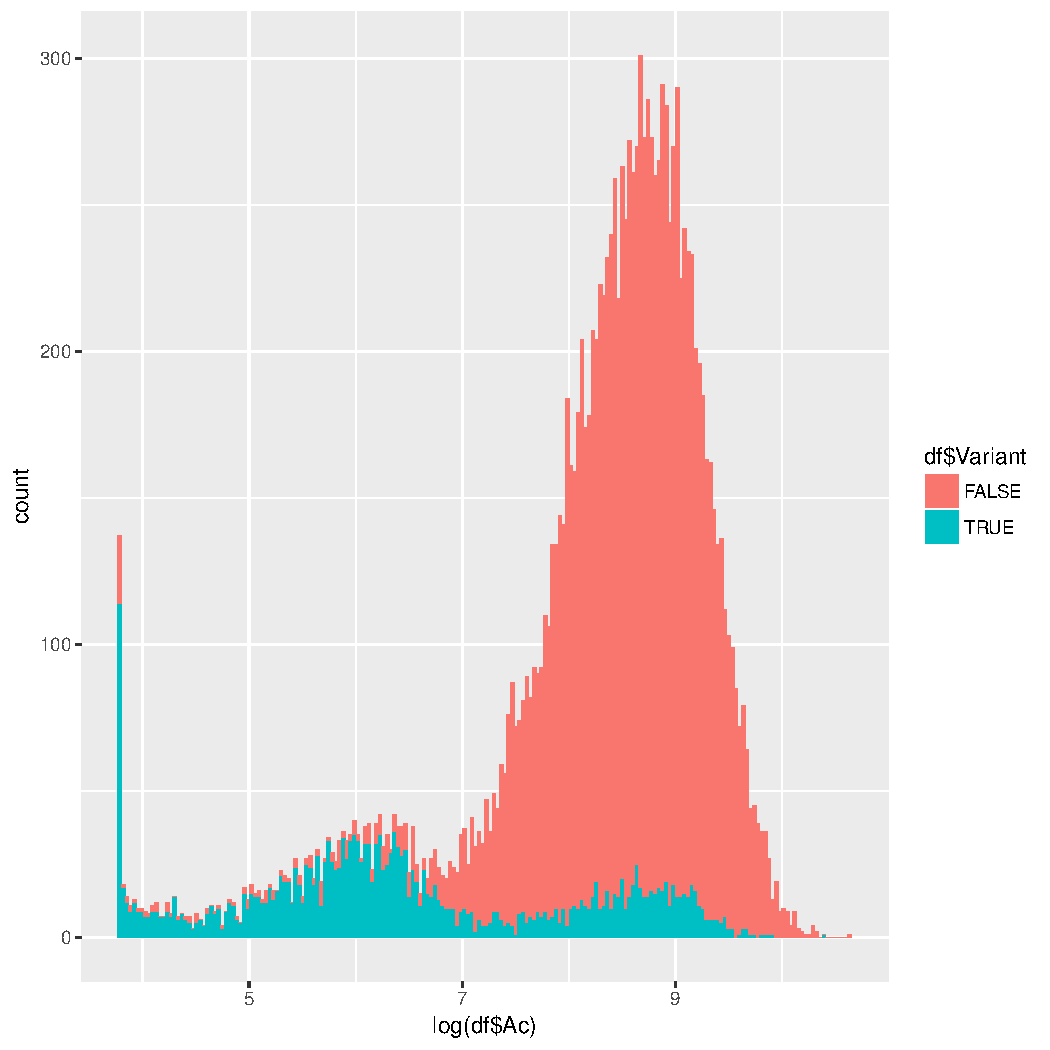
\includegraphics[width=1\linewidth]{figure/dens_3-1} 

\end{knitrout}
\begin{knitrout}
\definecolor{shadecolor}{rgb}{0.969, 0.969, 0.969}\color{fgcolor}\begin{kframe}
\begin{alltt}
\hlkwd{table}\hlstd{(cov}\hlopt{$}\hlstd{Variant)}
\end{alltt}
\begin{verbatim}
## 
##  FALSE   TRUE 
## 110292   6365
\end{verbatim}
\begin{alltt}
\hlcom{#df <- cov }
\hlstd{df} \hlkwb{<-} \hlkwd{rbind}\hlstd{(}\hlkwd{sample_n}\hlstd{(cov[cov}\hlopt{$}\hlstd{Variant} \hlopt{==} \hlnum{FALSE}\hlstd{,],} \hlnum{6365}\hlstd{), cov[cov}\hlopt{$}\hlstd{Variant} \hlopt{==} \hlnum{TRUE}\hlstd{,])}

\hlstd{train_idx} \hlkwb{<-} \hlkwd{rownames}\hlstd{(}\hlkwd{sample_n}\hlstd{(df,} \hlnum{8486}\hlstd{))}
\hlstd{train_df} \hlkwb{<-} \hlstd{df[}\hlkwd{rownames}\hlstd{(df)} \hlopt \hlstd{train_idx,]}
\hlstd{test_df} \hlkwb{<-} \hlstd{df[}\hlopt{!}\hlkwd{rownames}\hlstd{(df)} \hlopt \hlstd{train_idx,]}

\hlstd{model} \hlkwb{<-} \hlkwd{glm}\hlstd{(Variant} \hlopt{~} \hlstd{Ac}\hlopt{+}\hlstd{Met}\hlopt{+}\hlstd{Type,} \hlkwc{family}\hlstd{=}\hlkwd{binomial}\hlstd{(}\hlkwc{link}\hlstd{=}\hlstr{'logit'}\hlstd{),}\hlkwc{data}\hlstd{=train_df)}
\hlkwd{summary}\hlstd{(model)}
\end{alltt}
\begin{verbatim}
## 
## Call:
## glm(formula = Variant ~ Ac + Met + Type, family = binomial(link = "logit"), 
##     data = train_df)
## 
## Deviance Residuals: 
##     Min       1Q   Median       3Q      Max  
## -4.9780  -0.8216  -0.0517   0.3802   3.5533  
## 
## Coefficients:
##               Estimate Std. Error z value Pr(>|z|)    
## (Intercept) -1.519e+00  1.214e-01 -12.513  < 2e-16 ***
## Ac          -1.103e-04  9.176e-06 -12.018  < 2e-16 ***
## Met          1.873e-04  7.302e-06  25.651  < 2e-16 ***
## Type5prima  -5.411e-01  1.572e-01  -3.443 0.000575 ***
## TypeORF      1.375e+00  1.167e-01  11.783  < 2e-16 ***
## Typeother   -3.570e+00  3.848e-01  -9.278  < 2e-16 ***
## ---
## Signif. codes:  0 '***' 0.001 '**' 0.01 '*' 0.05 '.' 0.1 ' ' 1
## 
## (Dispersion parameter for binomial family taken to be 1)
## 
##     Null deviance: 11764.1  on 8485  degrees of freedom
## Residual deviance:  6670.4  on 8480  degrees of freedom
## AIC: 6682.4
## 
## Number of Fisher Scoring iterations: 7
\end{verbatim}
\begin{alltt}
\hlstd{fitted.results} \hlkwb{<-} \hlkwd{predict}\hlstd{(model, test_df,} \hlkwc{type}\hlstd{=}\hlstr{'response'}\hlstd{)}
\hlkwd{table}\hlstd{(test_df}\hlopt{$}\hlstd{Variant, fitted.results} \hlopt{>} \hlnum{0.5}\hlstd{)}
\end{alltt}
\begin{verbatim}
##        
##         FALSE TRUE
##   FALSE  2071   48
##   TRUE    689 1436
\end{verbatim}
\begin{alltt}
\hlstd{fitted.results} \hlkwb{<-} \hlkwd{ifelse}\hlstd{(fitted.results} \hlopt{>} \hlnum{0.5}\hlstd{,}\hlnum{1}\hlstd{,}\hlnum{0}\hlstd{)}
\hlstd{misClasificError} \hlkwb{<-} \hlkwd{mean}\hlstd{(fitted.results} \hlopt{!=} \hlstd{test_df}\hlopt{$}\hlstd{Variant)}
\hlkwd{print}\hlstd{(}\hlkwd{paste}\hlstd{(}\hlstr{'Accuracy'}\hlstd{,}\hlnum{1}\hlopt{-}\hlstd{misClasificError))}
\end{alltt}
\begin{verbatim}
## [1] "Accuracy 0.826343072573044"
\end{verbatim}
\begin{alltt}
\hlstd{test_df[}\hlstr{"Pred"}\hlstd{]} \hlkwb{<-} \hlstd{fitted.results}
\hlstd{test_df[}\hlstr{"all_0"}\hlstd{]} \hlkwb{<-} \hlnum{0}
\hlstd{misClasificError2} \hlkwb{<-} \hlkwd{mean}\hlstd{(test_df}\hlopt{$}\hlstd{all_0} \hlopt{!=} \hlstd{test_df}\hlopt{$}\hlstd{Variant)}
\hlkwd{print}\hlstd{(}\hlkwd{paste}\hlstd{(}\hlstr{'Accuracy of null model'}\hlstd{,}\hlnum{1}\hlopt{-}\hlstd{misClasificError2))}
\end{alltt}
\begin{verbatim}
## [1] "Accuracy of null model 0.499293119698398"
\end{verbatim}
\begin{alltt}
\hlkwd{library}\hlstd{(ROCR)}
\end{alltt}


{\ttfamily\noindent\itshape\color{messagecolor}{\#\# Loading required package: gplots}}

{\ttfamily\noindent\itshape\color{messagecolor}{\#\# \\\#\# Attaching package: 'gplots'}}

{\ttfamily\noindent\itshape\color{messagecolor}{\#\# The following object is masked from 'package:stats':\\\#\# \\\#\#\ \ \ \  lowess}}\begin{alltt}
\hlstd{predict} \hlkwb{<-} \hlkwd{predict}\hlstd{(model,} \hlkwc{type} \hlstd{=} \hlstr{'response'}\hlstd{)}
\hlstd{ROCRpred} \hlkwb{<-} \hlkwd{prediction}\hlstd{(predict, train_df}\hlopt{$}\hlstd{Variant)}
\hlstd{ROCRperf} \hlkwb{<-} \hlkwd{performance}\hlstd{(ROCRpred,} \hlstr{'tpr'}\hlstd{,}\hlstr{'fpr'}\hlstd{)}
\hlkwd{plot}\hlstd{(ROCRperf,} \hlkwc{colorize} \hlstd{=} \hlnum{TRUE}\hlstd{,} \hlkwc{text.adj} \hlstd{=} \hlkwd{c}\hlstd{(}\hlopt{-}\hlnum{0.2}\hlstd{,}\hlnum{1.7}\hlstd{))}
\end{alltt}
\end{kframe}
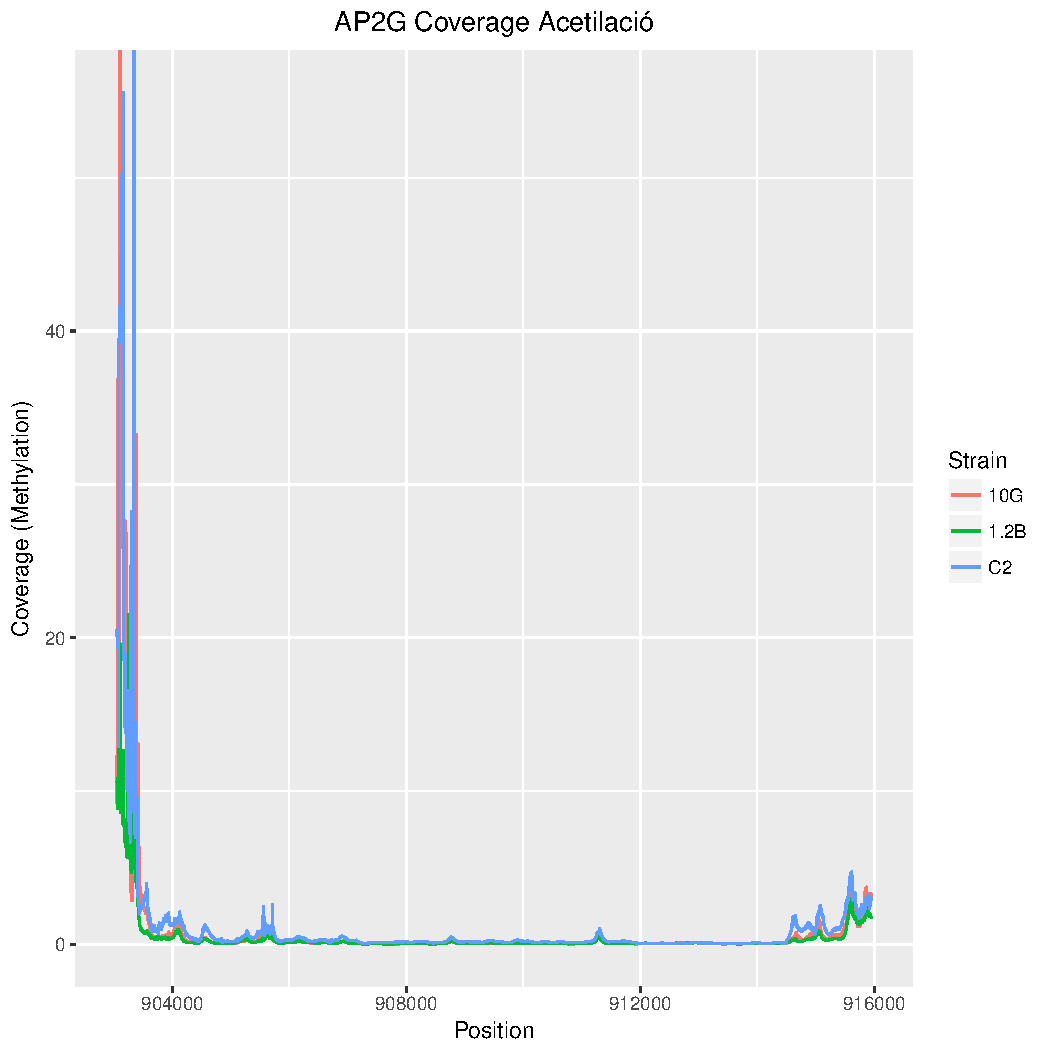
\includegraphics[width=\maxwidth]{figure/unnamed-chunk-1-1} 
\begin{kframe}\begin{alltt}
\hlstd{false_pos_idx} \hlkwb{<-} \hlkwd{rownames}\hlstd{(test_df[test_df}\hlopt{$}\hlstd{Pred} \hlopt{==} \hlnum{1} \hlopt{&} \hlstd{test_df}\hlopt{$}\hlstd{Variant} \hlopt{==} \hlnum{FALSE}\hlstd{,])}
\hlstd{false_pos} \hlkwb{<-} \hlstd{cov[}\hlkwd{rownames}\hlstd{(cov)} \hlopt \hlstd{false_pos_idx,]}
\hlkwd{table}\hlstd{(false_pos}\hlopt{$}\hlstd{Type)}
\end{alltt}
\begin{verbatim}
## 
## 3prima 5prima    ORF  other 
##     14     19     10      5
\end{verbatim}
\begin{alltt}
\hlstd{false_neg_idx} \hlkwb{<-} \hlkwd{rownames}\hlstd{(test_df[test_df}\hlopt{$}\hlstd{Pred} \hlopt{==} \hlnum{0} \hlopt{&} \hlstd{test_df}\hlopt{$}\hlstd{Variant} \hlopt{==} \hlnum{TRUE}\hlstd{,])}
\hlstd{false_neg} \hlkwb{<-} \hlstd{cov[}\hlkwd{rownames}\hlstd{(cov)} \hlopt \hlstd{false_neg_idx,]}
\hlkwd{table}\hlstd{(false_neg}\hlopt{$}\hlstd{Type)}
\end{alltt}
\begin{verbatim}
## 
## 3prima 5prima    ORF  other 
##     51     60    572      6
\end{verbatim}
\end{kframe}
\end{knitrout}

\end{document}
